\documentclass[letterpaper,11pt]{article}
\oddsidemargin -1.0cm \textwidth 17.5cm

\usepackage[utf8]{inputenc}
\usepackage[activeacute,spanish, es-lcroman]{babel}
\decimalpoint
\usepackage{amsfonts,setspace}
\usepackage{amsmath}
\usepackage{amssymb, amsmath, amsthm}
\usepackage{comment}
\usepackage{float}
\usepackage{amssymb}
\usepackage{dsfont}
\usepackage{anysize}
\usepackage{multicol}
\usepackage{enumerate}
\usepackage{graphicx}
\usepackage[left=1.5cm,top=2cm,right=1.5cm, bottom=1.7cm]{geometry}
\setlength\headheight{1.5em} 
\usepackage{fancyhdr}
\usepackage{multicol}
\usepackage{hyperref}
\usepackage{wrapfig}
\usepackage{subcaption}
\usepackage{siunitx}
\usepackage{cancel}
\usepackage{mdwlist}
\usepackage{svg}
\pagestyle{fancy}
\fancyhf{}
\renewcommand{\labelenumi}{\normalsize\bfseries P\arabic{enumi}.}
\renewcommand{\labelenumii}{\normalsize\bfseries (\alph{enumii})}
\renewcommand{\labelenumiii}{\normalsize\bfseries \roman{enumiii})}


\begin{document}

\fancyhead[L]{\itshape{Facultad de Ciencias F\'isicas y Matem\'aticas}}
\fancyhead[R]{\itshape{Universidad de Chile}}
\rfoot[]{pág. \thepage}

\begin{minipage}{11.5cm}
    \begin{flushleft}
        \hspace*{-0.6cm}\textbf{FI1000-1 Introducción a la Física Clásica}\\
        \hspace*{-0.6cm}\textbf{Profesor:} Ignacio Bordeu\\
        \hspace*{-0.6cm}\textbf{Auxiliares:} Alejandro Cartes \& Simón Yáñez\\
        \hspace*{-0.6cm}\textbf{Ayudante:} Javier Cubillos\\
    \end{flushleft}
\end{minipage}

\begin{picture}(2,3)
    \put(366, 10){
\includegraphics[scale=0.9]{2020-1/Imágenes/logo/dfi-fcfm.pdf}}
\end{picture}

\begin{center}
	\LARGE\textbf{Auxiliar \#7}\\
	\Large{Resortes}
\end{center}

\vspace{-1cm}
\begin{enumerate}\setlength{\itemsep}{0.4cm}

\item[]

\item Considere dos bloques de masa $m$ unidos por un resorte de constante elástica $k$. El sistema formado por los dos bloques y el resorte descansa en forma vertical sobre una mesa tal como se indica en la figura ¿En cuánto debe comprimirse el resorte con respecto al largo natural para que al soltar el sistema éste eventualmente despegue de la mesa?

    \begin{figure}[H]
        \centering
        \svgpath{../../2023-1/img/aux_7/}
        \includesvg[width=0.75\linewidth]{Aux 7 - P1.svg}
    \end{figure}
\item
Una argolla de masa $M$ está inserta en un alambre vertical. El coeficiente de roce estático entre el alambre y la argolla es $\mu_e$. La argolla está conectada a un resorte de constante elástica k y largo natural despreciable. El extremo fijo del resorte está a una distancia $b$ del alambre. Determinar los valores posibles de $M$ para que la argolla se mantenga a una distancia $h$ del techo.
        

    \begin{figure}[H]
        \centering
        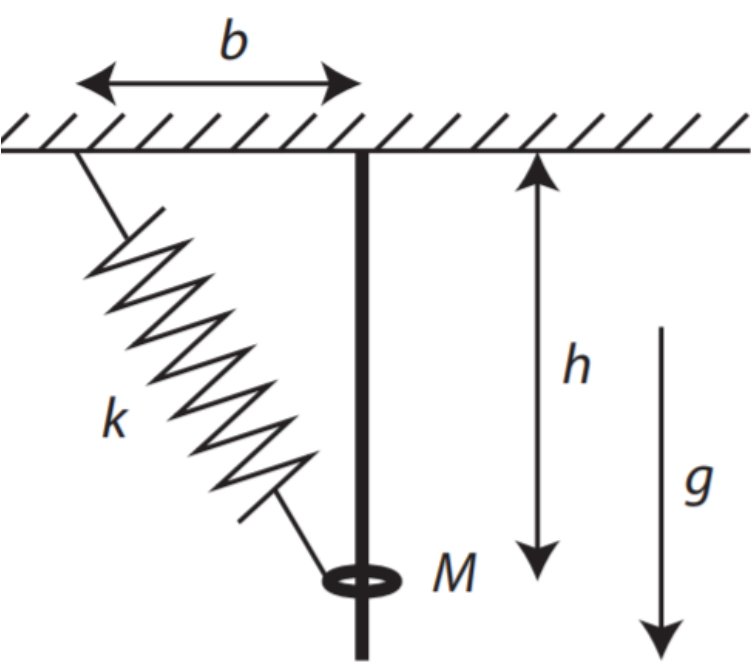
\includegraphics[width=0.4\textwidth]{2023-1/img/aux_7/Aux 7 - P2.PNG}
    \end{figure}
    
    
\newpage

\item En el sistema de la figura aparecen dos resortes idénticos unidos en el extremo común por un anillo de masa $M$. este anillo se puede deslizar sin roce a lo largo de la barra horizontal. No considere el peso del
anillo. Encuentre el punto de equilibrio (el valor de $x$) del sistema de resortes para los casos:

\begin{enumerate}   
    \begin{multicols}{3}
    \item $l<a$
    \columnbreak
    \item $l=a$
    \columnbreak
    \item $l>a$
    \end{multicols}
\end{enumerate}
    \begin{figure}[H]
        \centering
        \svgpath{../../2023-1/img/aux_7/}
        \includesvg[width=0.9\linewidth]{Aux 7 - P3.svg}
    \end{figure}

% Para imágenes vectoriales -> el texto tiene que estar en LaTeX
% \begin{figure}[htbp]
%   \centering
%   \svgpath{../Imagenes/ejercicios}  -> .. irse pa'trás 
%   \includesvg{ej5.svg}
% \end{figure}
\end{enumerate}
\end{document}